\documentclass[10pt]{beamer}

\usetheme[progressbar=frametitle]{metropolis}
\usepackage{appendixnumberbeamer}

\usepackage{booktabs}
\usepackage[scale=2]{ccicons}

\usepackage{pgfplots}
\usepgfplotslibrary{dateplot}

\usepackage{xspace}
\newcommand{\themename}{\textbf{\textsc{metropolis}}\xspace}


\usepackage[bookmarksopen=true]{hyperref}
\usepackage{xcolor}
\usepackage{graphicx}
\usepackage[group-separator = {,}]{siunitx}


\newcommand{\faro}[0]{FARO\textsuperscript{\textregistered}}

% Use metropolis theme
\title{Hyper Parameter Optimization \\using Machine Learning}
\date{July, 2021}
\author{{Nuno Costa} \\
{\textit{ISEP Advisor}: Carlos Ramos} \\
{\textit{External Advisor}: Hooshiar Zolfagharnasab}}
\institute{Polytechnic of Porto - School of Engineering (ISEP)}


\begin{document}

  \maketitle
  \section[agenda]
  \section{Introduction}
  \begin{frame}{\faro Overview}
    \begin{columns}
      \begin{column}{0.6\textwidth}
        \faro is a market leader in the 3D metrology market with over \SI{150}[US\$]{M} of gross profit in 2020. It produces a large variety of devices (contact and non-contact measurement arms, laser scanners) and a suite of software products which integrate the devices into the customers workflow.
      \end{column}
      \begin{column}{0.5\textwidth}
        \begin{figure}[r]
        \centering
        
\includegraphics[width=0.7\textwidth]{images/faro_logo.png}
        \end{figure}
      \end{column}
    \end{columns}
  \end{frame}

  \begin{frame}{\faro Devices}
    \begin{columns}
      \begin{column}{0.35\textwidth}
        \begin{figure}
          \centering
          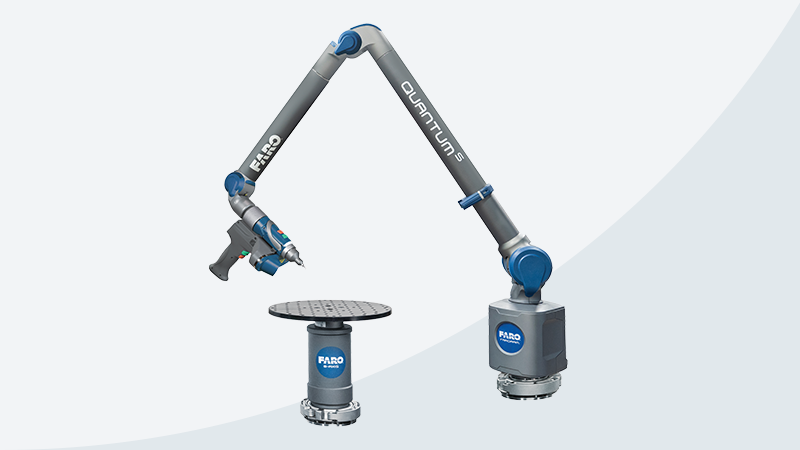
\includegraphics[width=\textwidth]{images/faro_quantum_s_arm.png}
          \caption{\\\faro Quantum S Arm}
        \end{figure}
      \end{column}
      \begin{column}{0.35\textwidth}
        \begin{figure}
          \centering
          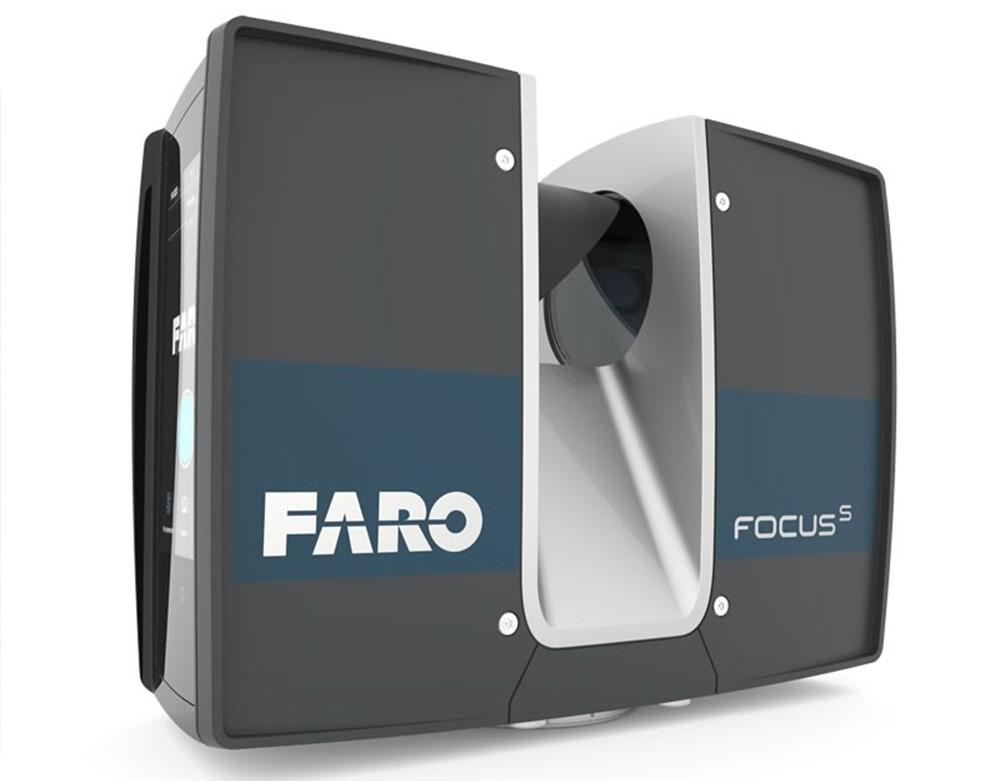
\includegraphics[width=0.8\textwidth]{images/faro_scanner.jpg}
          \caption{\\\faro Focus Laser Scanner}
        \end{figure}
      \end{column}
      \begin{column}{0.35\textwidth}
        \begin{figure}
          \centering
          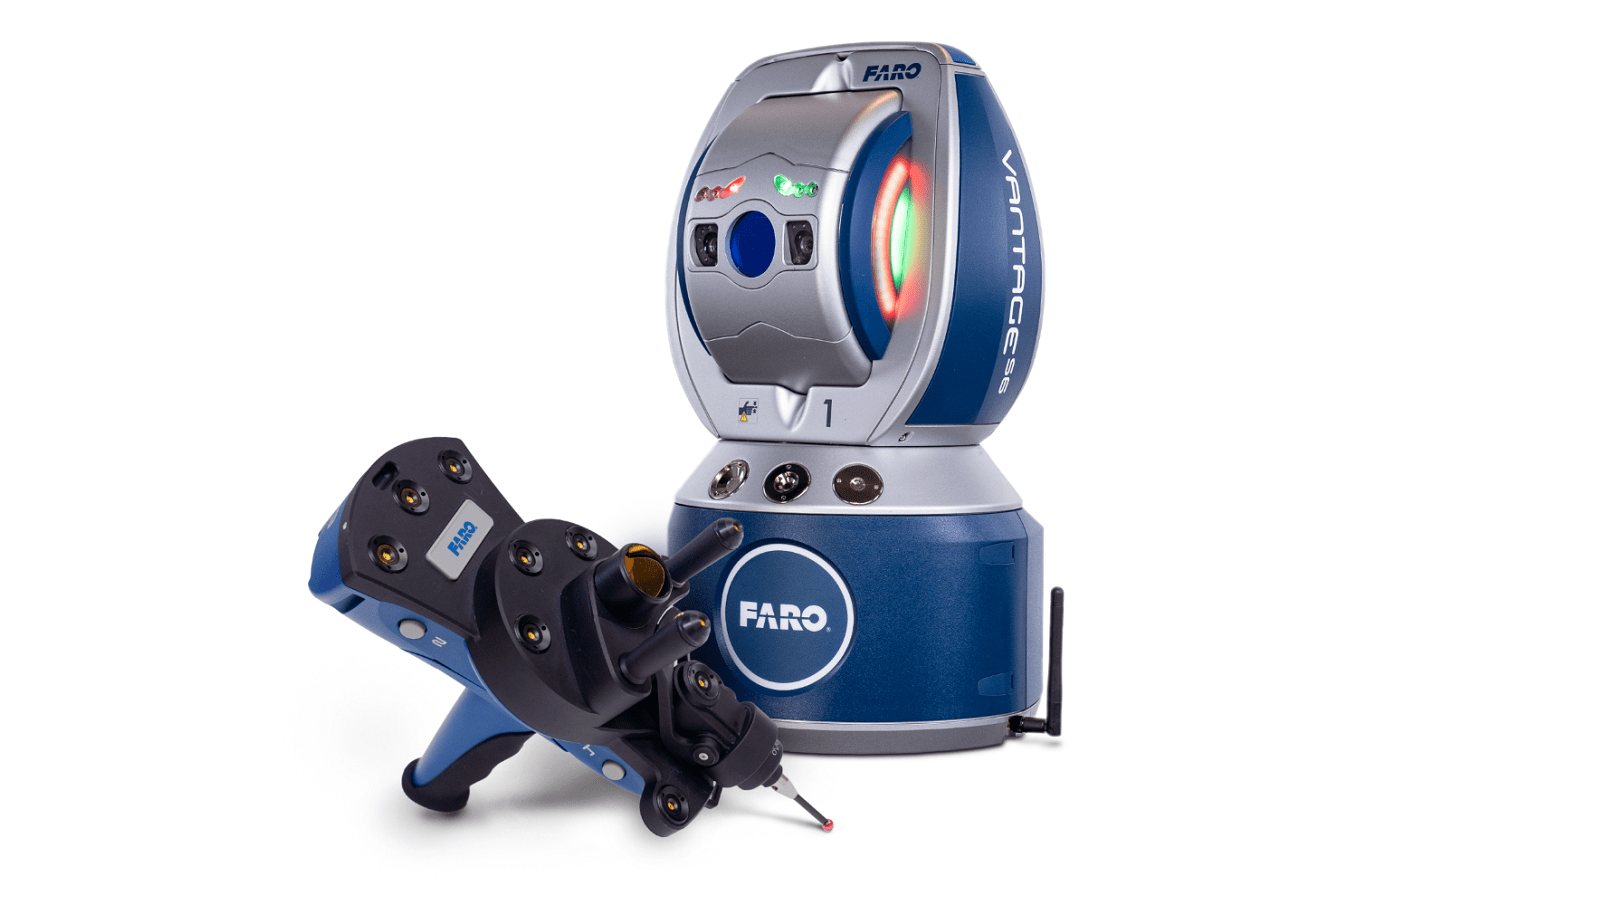
\includegraphics[width=\textwidth]{images/faro-probe.png}
          \caption{\\\faro Vantage Laser Tracker}
        \end{figure}
      \end{column}
    \end{columns}
  \end{frame}

  \begin{frame}{Problem Description}
    \faro is investing heavily  in machine learning within its software suite. As such, there is a need for algorithm training tools that integrate into \faro's codebase.

    This project focuses on demonstrating successful usage of these tools with \faro software, specifically a function within CAM2\textsuperscript{\textregistered}. 
  \end{frame}

  \begin{frame}{Objectives}
    The objective of this internship was to create a solution for hyper parameter optimization in software solutions developed by \faro. The main goals for this internship were to:
    \begin{itemize}
      \item Develop 3 algorithm training solutions
      \item Develop meaningful unit tests for these solutions
      \item Integrate the solutions into pre-existing software
      \item Demonstrate value by solving real world issues in CAM2\textsuperscript{\textregistered} software
    \end{itemize}
  \end{frame}

  \section{State of the Art}
  \subsection{Related Works}
  \begin{frame}{Related Works}
    With regards to related works, we have explored the existing field of hyper parameter optimization. This field has a long history, dating back to the 1990s.
  \end{frame}
  \begin{frame}{Related Works}
    \begin{figure}
          \centering
          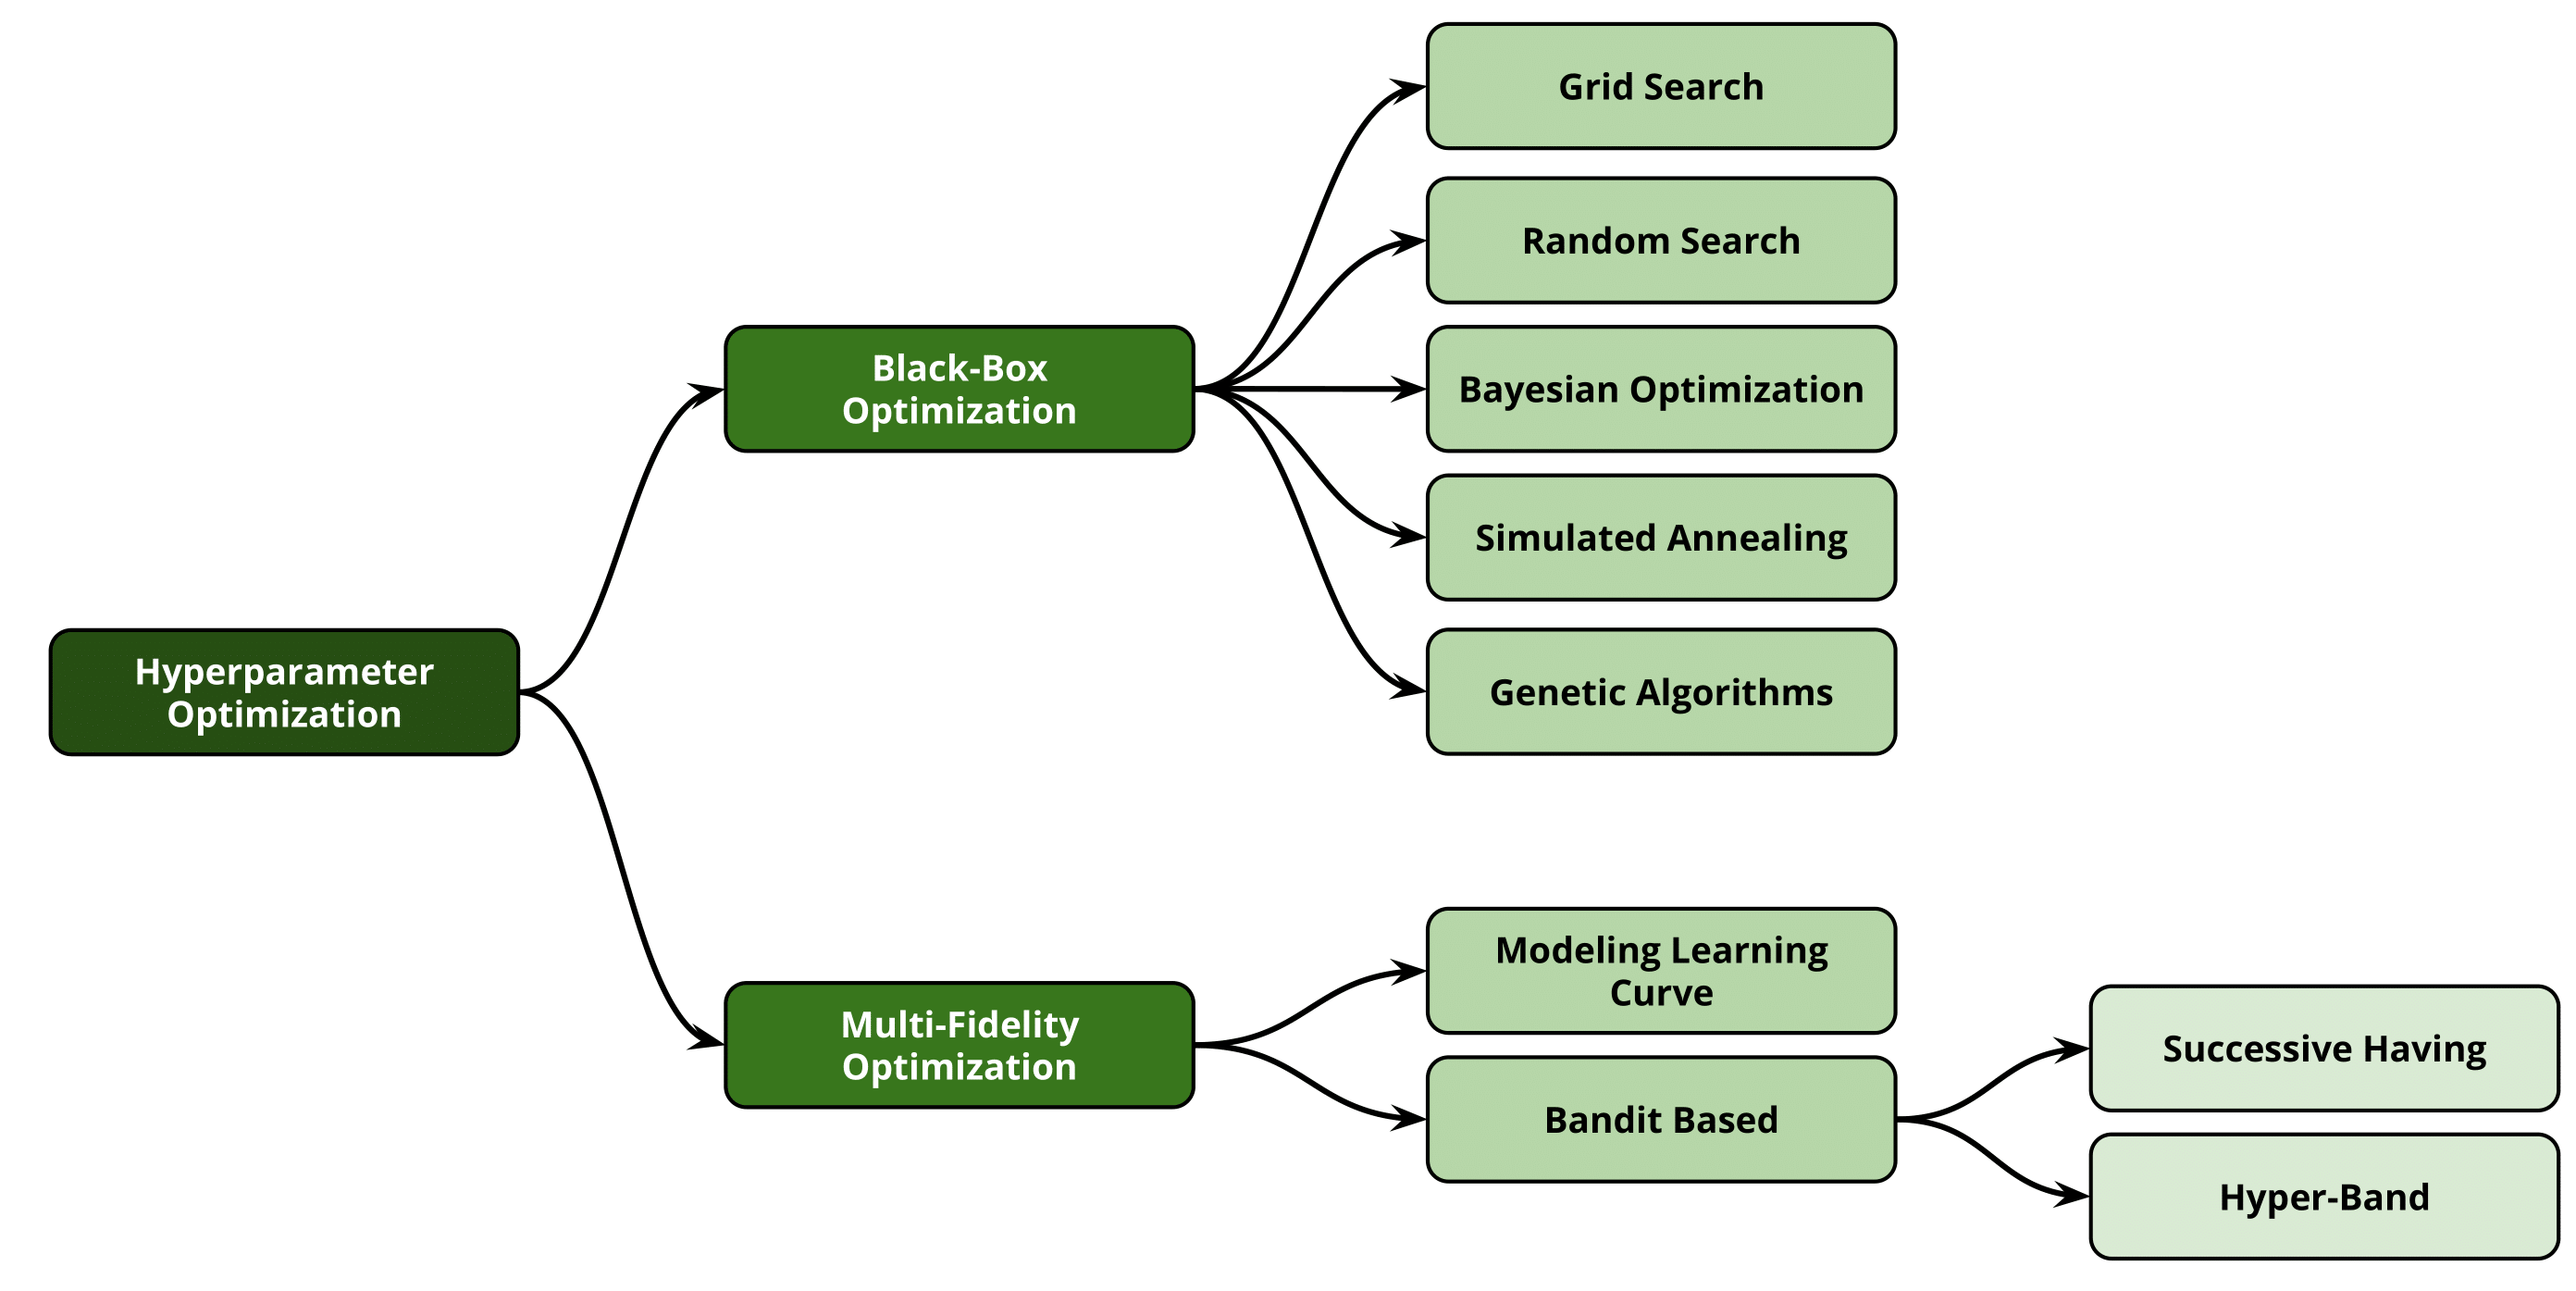
\includegraphics[width=\textwidth]{images/state_art-taxonomy_optimizers.png}
        \end{figure}
  \end{frame}
  \begin{frame}{Black-Box Optimization Algorithms}
    Hello, world!
  \end{frame}
  \begin{frame}{Multi-Fidelity Optimization Algorithms}
    Hello, world!
  \end{frame}
  \subsection{Existing Technologies}
  \begin{frame}{Existing Technologies}
    Hello, world!
  \end{frame}
  \begin{frame}{Hyper Parameter Optimization}
    Hello, world!
  \end{frame}
  \begin{frame}{Virtualization}
    Hello, world!
  \end{frame}
  \begin{frame}{Machine Learning Data Visualization}
    Hello, world!
  \end{frame}
\end{document}
